\documentclass{article}

\usepackage[a4paper]{geometry}
\usepackage[ngerman]{babel}
\usepackage[utf8]{inputenc}
\usepackage[T1]{fontenc}
\usepackage{graphicx}
\usepackage{fancyhdr}
\usepackage{xcolor}
\usepackage{float}
\usepackage{hyperref}

\graphicspath{{./images/}}

\pagestyle{fancyplain}
\fancyhf{}
\lhead{\fancyplain{}{Gruppe 11 – Mathias Baumbach \& Mara Schulke} }
\rhead{\fancyplain{}{\today}}
\cfoot{\fancyplain{}{\thepage}}

\begin{document}

\begin{titlepage}
	\begin{flushleft}
		TH Brandenburg \\
		Online Studiengang IT Sicherheit \\
		Fachbereich Informatik und Medien \\
		Netzwerksicherheit \\
		Prof.\ Dr.\ Michael Pilgermann
	\end{flushleft}

	\vfill

	\begin{center}
		\Large{Einsendeaufgabe 2}\\[0.5em]
		\large{Wintersemester 2023}\\[0.25em]
		\large{Abgabetermin \today}
	\end{center}

	\vfill

	\begin{flushright}
		Gruppe 11 \\
		Mathias Baumbach (Matr-Nr. 20213703) \\
		Mara Schulke (Matr-Nr. 20215853)
	\end{flushright}
\end{titlepage}

\begin{abstract}
\end{abstract}

\tableofcontents

\listoffigures

\newpage

\section{Durchführung}

\subsection{SSL Test I}

\subsubsection*{Aufgabenstellung}

Testen Sie den Server nwsmooc.mooin.org mit der SSL-Testseite von Qualys 
und erklären Sie die Ergebnisse (hinsichtlich Zertifikaten, TLS-Versionen,
Handshakes und Details der Protokolle). Erklären Sie für eine weitere
Webpräsenz, die als "Recent Worst" bewertet wird, was bei dieser nicht stimmt. 

Hinweis: "Recent Worst" ist eine Liste auf der rechten Seite der Testseite. Zur
besseren Nachvollziehbarkeit bitte Screenshots hinzufügen. Deren Inhalte sollen
aber jeweils von Ihnen erklärt werden.

\subsubsection*{Antwort}

\begin{figure}[H]
	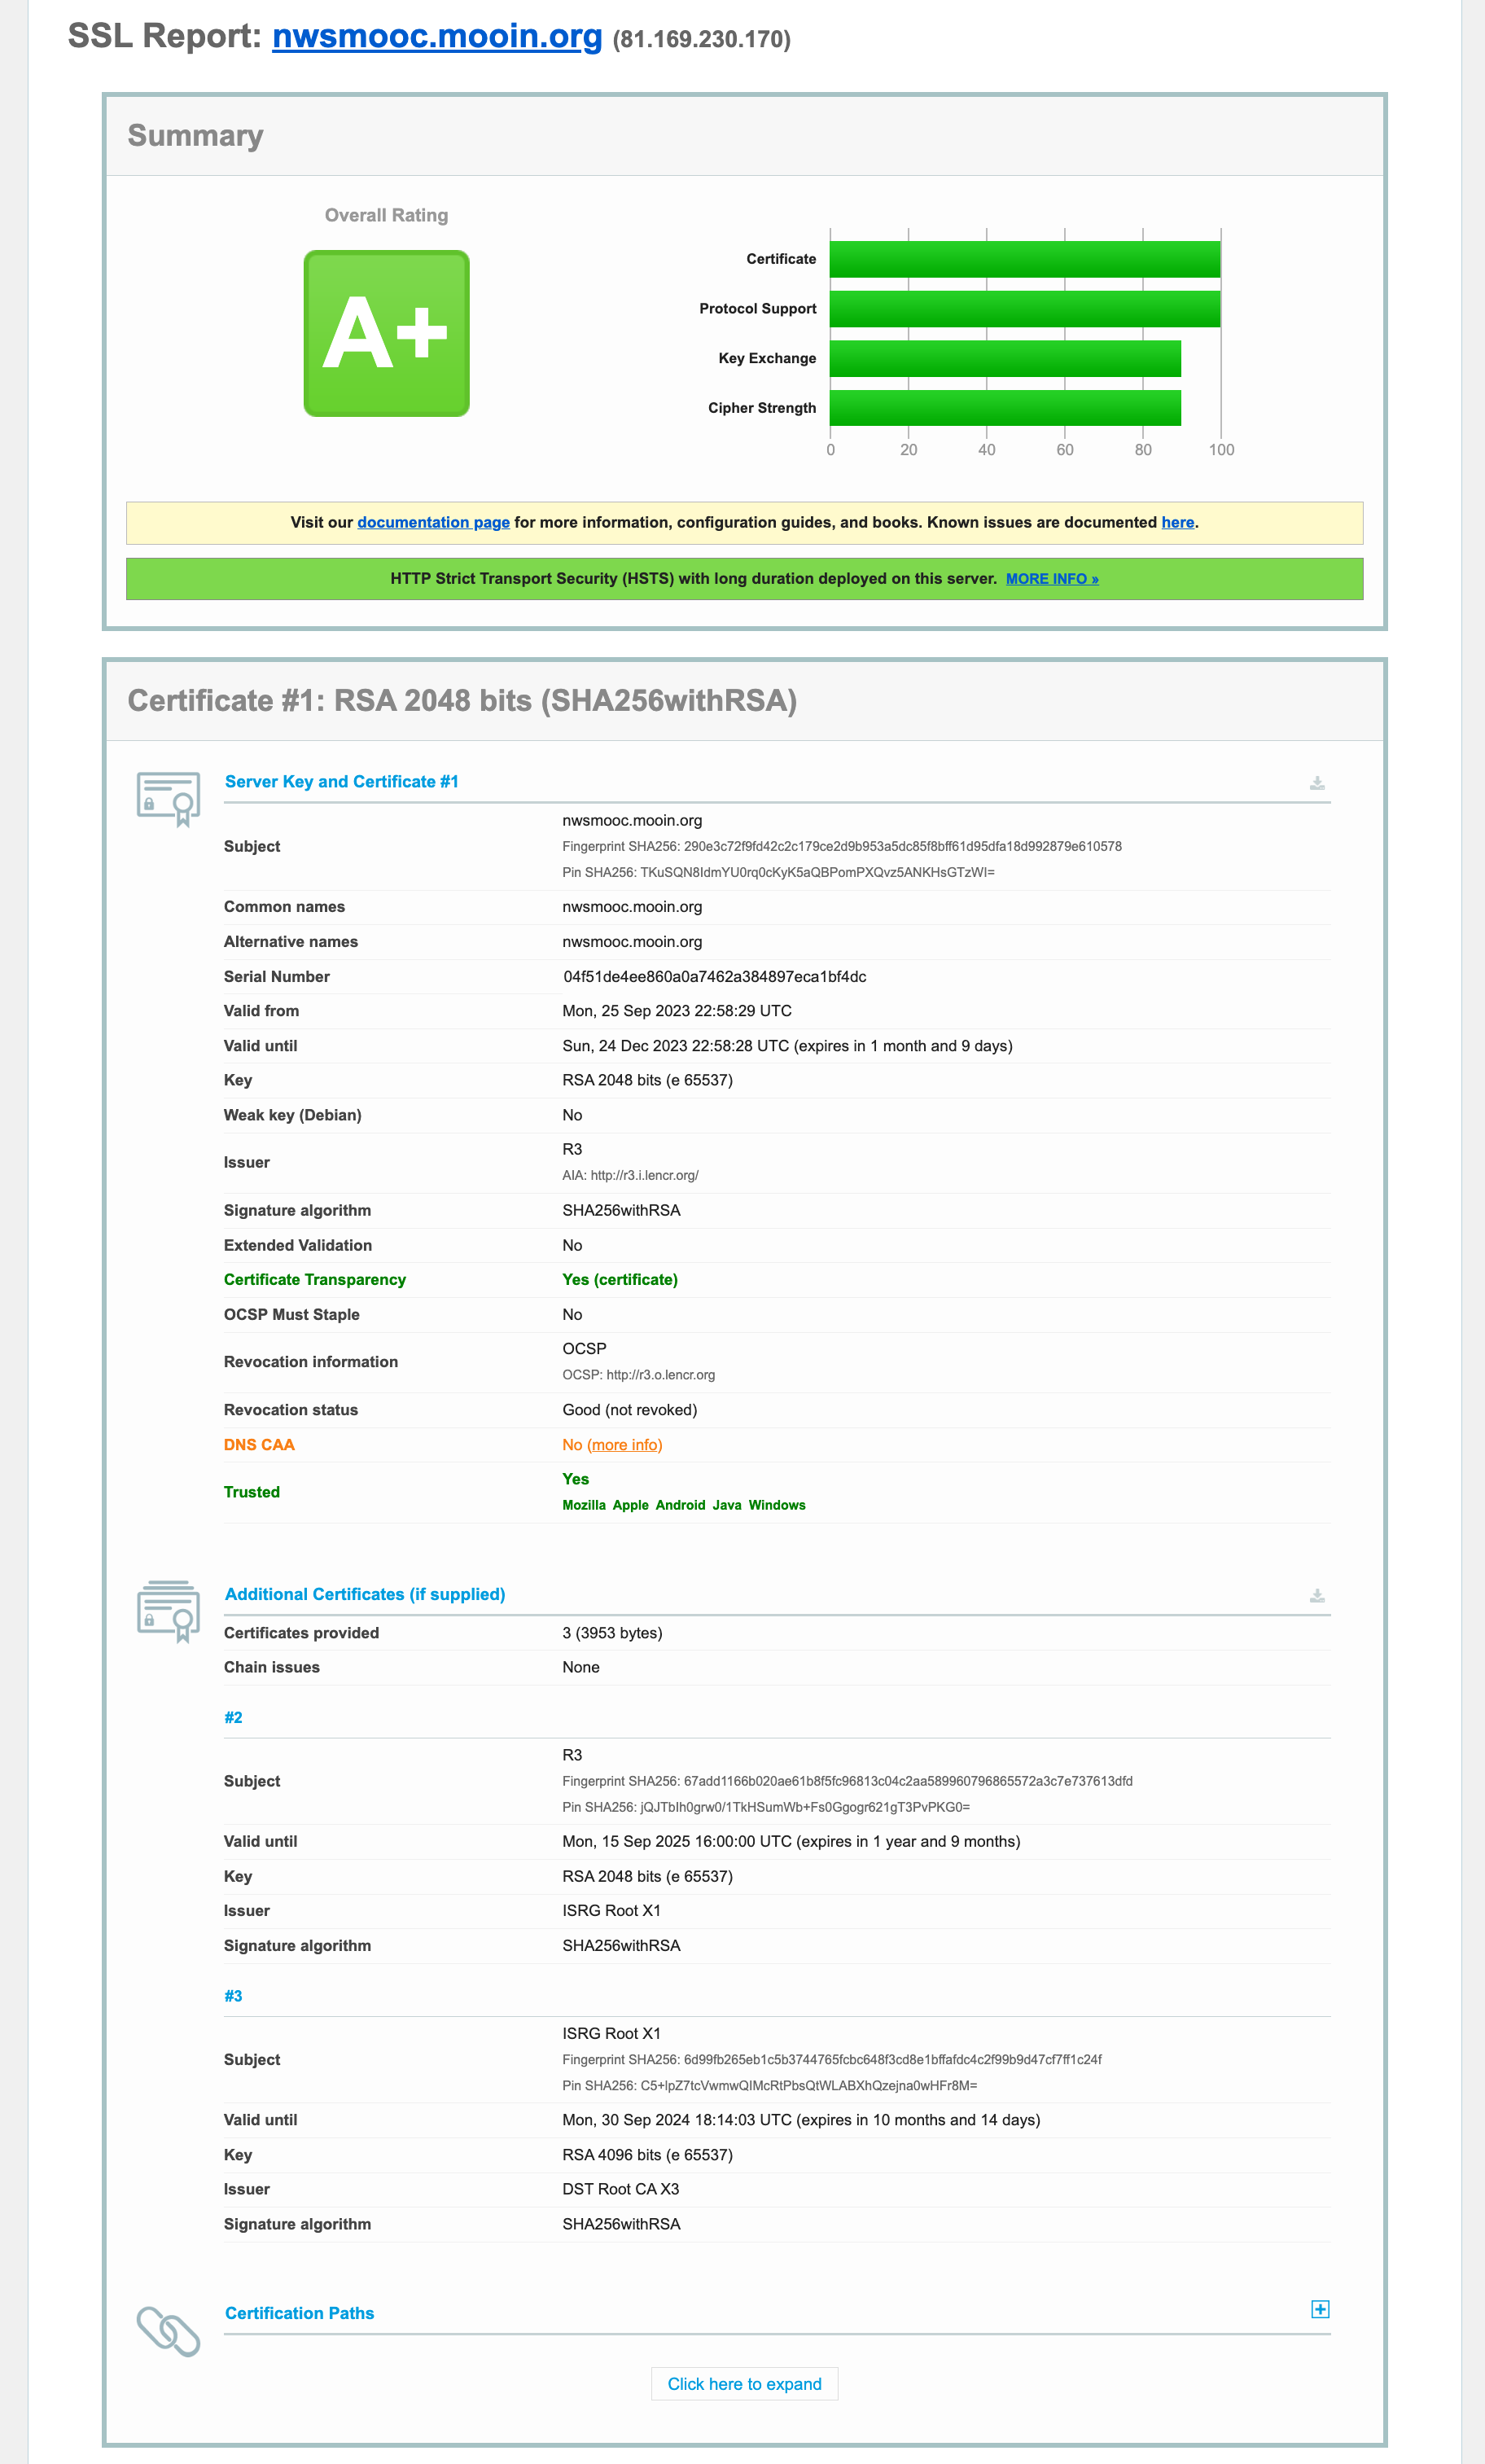
\includegraphics[width=0.75\textwidth]{images/01}
	\centering
	\caption{QualysSSL Test – nwsmooc.mooin.org}
\end{figure}

Der Web-Server hat insgesamt eine A+-Bewertung erhalten und ist dementsprechend auf dem aktuellen Stand / robust was die SSL-Konfiguration angeht.
Das Zertifikat des Servers ist ein 2048-Bit RSA-Zertifikat, das mit SHA256+RSA signiert wurde.
In dem Report von Qualys sind einige wichtige Eckdaten über das Zertifikat des Servers enthalten:

\begin{itemize}
    \item Gültigkeit: Von 25. September 2023 bis zum 24. Dezember 2023
    \item Aussteller: R3
    \item Status: Das Zertifikat wurde nicht widerrufen.
    \item Vertrauenswürdigkeit: Ja – Mozilla, Apple, Android, Java und Windows vertrauen diesem Zertifikat.
\end{itemize}

Außerdem gibt der Bericht die Zertifikate weiter oben in der Zertifikats-Kette an:

\begin{itemize}
    \item Zertifikat \#2: Aussteller R3, RSA 2048 Bit, gültig bis 15. September 2025.
    \item Zertifikat \#3: Aussteller ISRG Root X1, RSA 4096 Bit, gültig bis 30. September 2024.
\end{itemize}

\vspace{0.5em}

---

\begin{figure}[H]
	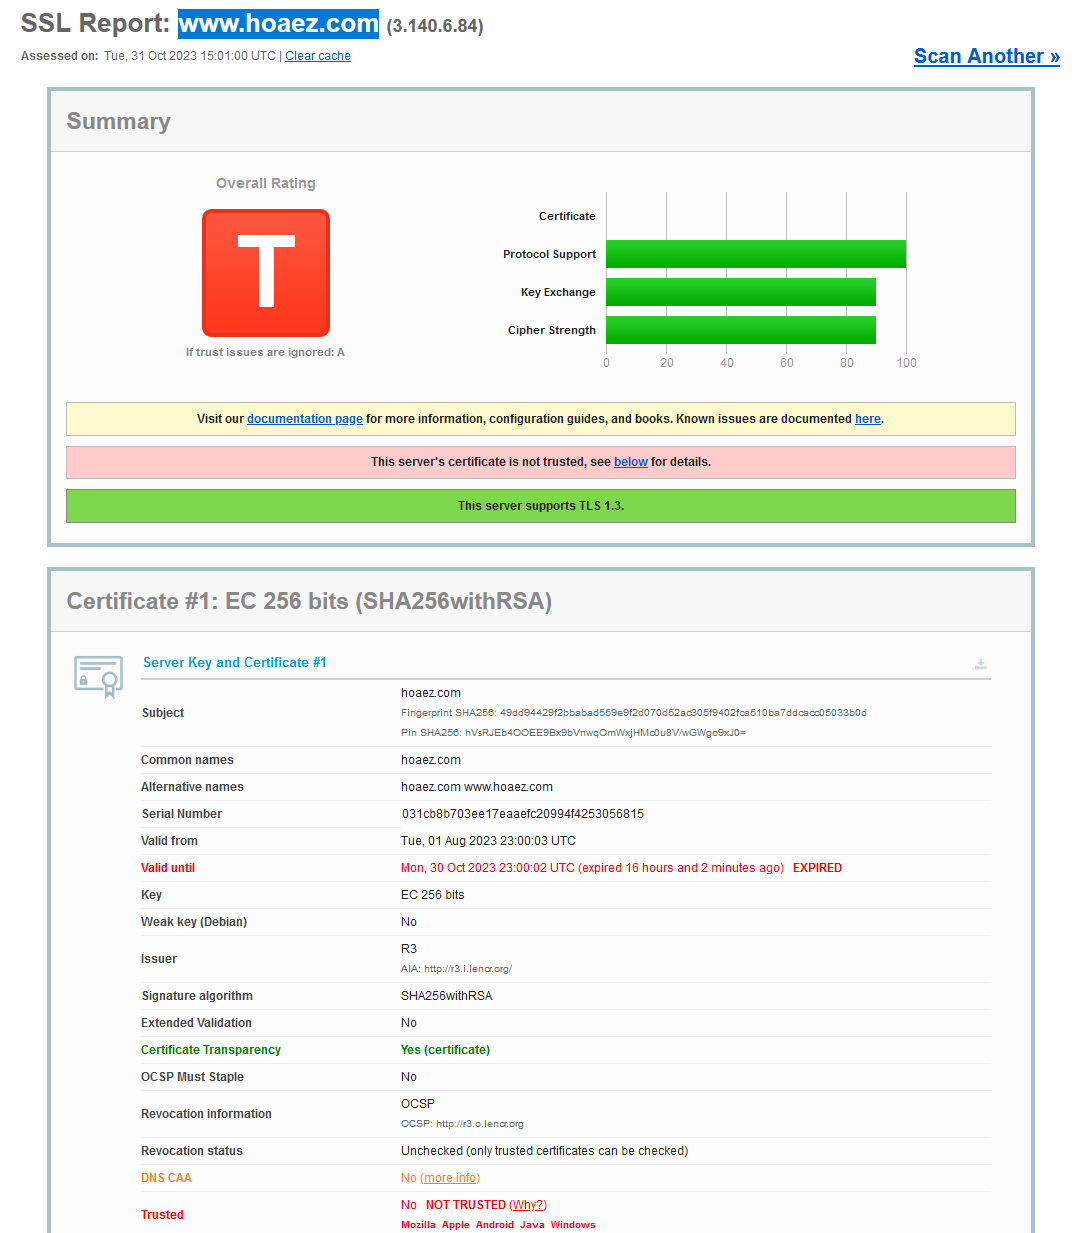
\includegraphics[width=0.75\textwidth]{images/02}
	\centering
	\caption{QualysSSL Test – Recent Worst}
\end{figure}

Der Server www.hoaez.com hat lediglich eine Gesamtbewertung von T erhalten, was bedeutet, dass dem Zertifikat
des Servers nicht vertraut werden kann (e.g. da es abgelaufen ist, oder durch eine Misskonfiguration). Um dennoch einen
Report erstellen zu können, hat Qualys die Vertrauenswürdigkeit bis auf weiteres ignoriert.


Unter der Zusammenfassung gibt es einen Abschnitt, der Details zum Zertifikat des Servers liefert. Diese deuten
explizit darauf hin, dass das Zertifikat (zum Test-Zeitpunkt seit 16 Stunden) abgelaufen und somit nicht mehr gültig ist.
Es ist anzunehmen, dass durch eine Erneuerung des Zertifikates, alle Probleme behoben werden können und der Server wieder
eine ausreichend gute Bewertung erhalten würde.

Das Zertifikat an sich ist verwendet Elliptic-Curve mit 256 Bits und wurde ebenfalls mit SHA256+RSA signiert.

Dieser Report ist ein gutes Beispiel dafür, als Administrator im Idealfall auf sich-selbsterneuernde Zertifikate zu setzen,
um einem Vertrauensverlust der Nutzer (durch eine Warnmeldung des Browsers) entgegen zu wirken.

\newpage

\subsection{SSL Test II}

\subsubsection*{Aufgabenstellung}

Führen Sie den Client-Test von Qualys aus und erklären Sie die Ergebnisse. (Siehe \url{https://clienttest.ssllabs.com:8443/ssltest/viewMyClient.html})

\subsubsection*{Antwort}

Wir haben den Client-Test mit der Mozilla Firefox Version 119.0.1 durchgeführt und folgendes Ergebnis erhalten:

\begin{figure}[H]
	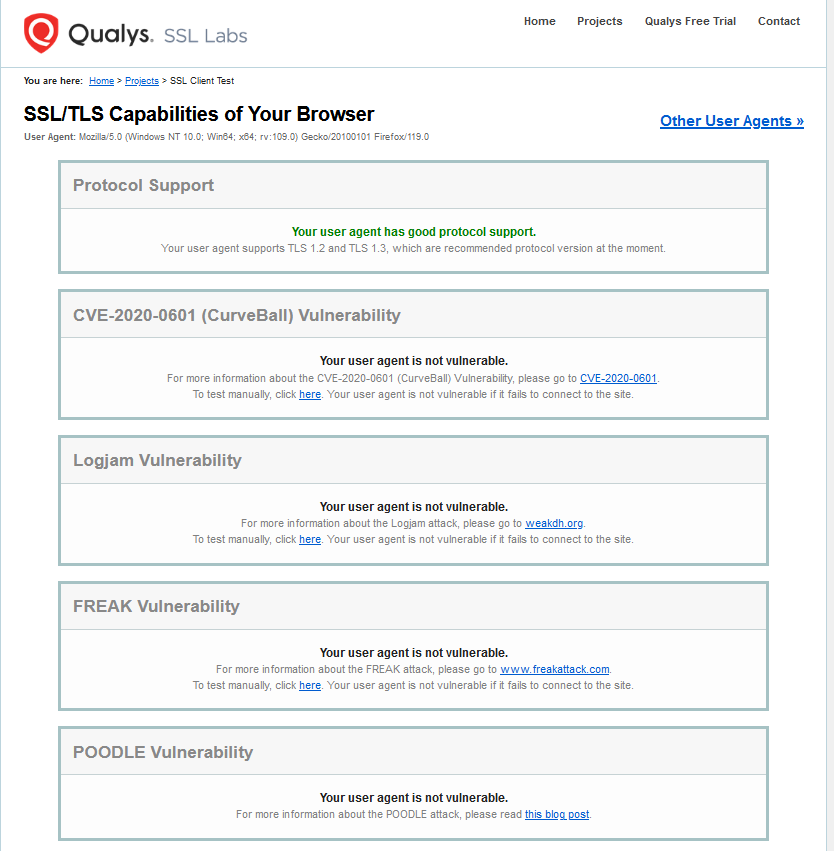
\includegraphics[width=0.75\textwidth]{images/03}
	\centering
	\caption{QualysSSL Test – Browser Capabilities}
\end{figure}

Im Kopf der Ergebnisseite wird eine Zusammenfassung der Bewertung ausgegeben. Es wird zunächst 
die Protokoll-Unterstützung mit grün/gut bewertet – in unserem Fall ob TLS 1.2 und TLS 1.3 unterstützt wird.
Danach folgen spezifische Schwachstellentests:

\begin{itemize}
    \item \textbf{Curveball / CVE-2020-0601} - Schwachstelle im Windows-OS bei der
    	Validierung von digitalen Zertifikaten die potentiell angreifbar für MitM macht.
    \item \textbf{Logjam} - Sicherheitslücke im Diffie-Hellman-Schlüsselaustausch,
		welcher bei verschlüsselten Verbindungen wie TLS verwendet wird. Ermöglicht den Schlüsselaustausch
		zu manipulieren und verschlüsselte Verbindungen zu entschlüsseln.
    \item \textbf{FREAK (Factoring RSA Export Keys)} – Sicherheitslücke, die Angreifern
		es ermöglichte Verschlüsselung von HTTPS-Verbindungen zu umgehen.
    \item \textbf{POODLE (Padding Oracle On Downgraded Legacy Encryption)} - Schwachstelle
		in SSLv2/3 die es ermöglichte die Verschlüsselung zu umgehen.
\end{itemize}

Keine der Schwachstellen sind auf unserem Client vorhanden.

\begin{figure}[H]
	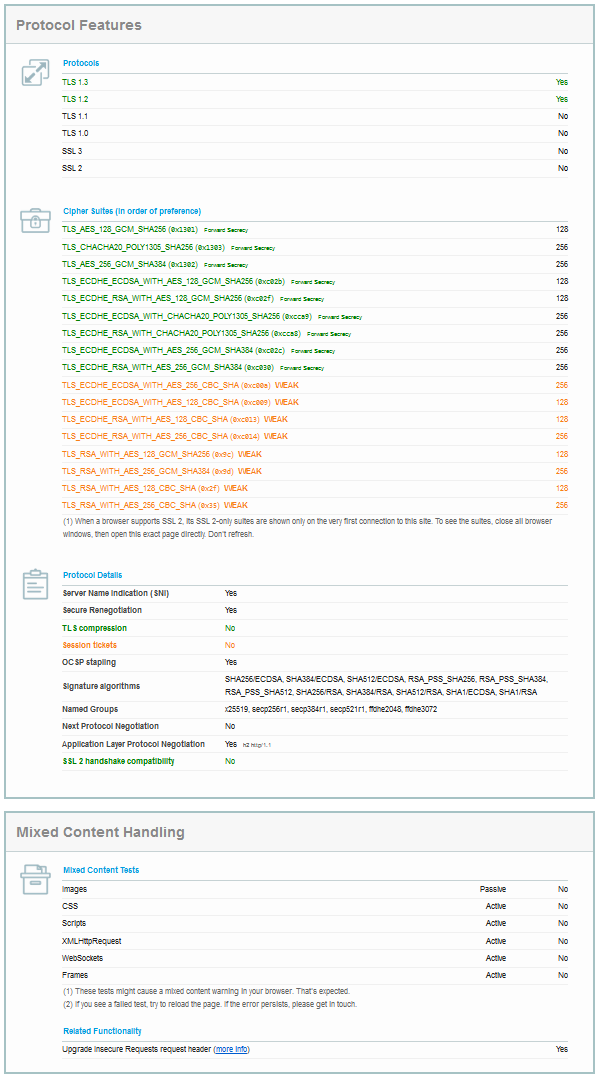
\includegraphics[width=0.75\textwidth]{images/04}
	\centering
	\caption{QualysSSL Test – Browser Protocol Features}
\end{figure}

Es folgt eine Detailauflistung der Protokoll-Features, die ergänzt ist um eine Auflistung der 
unterstützten Cipher Suites in Reihenfolge der Präferenz (von oben nach unten). Dabei werden viele 
kryptographische Verfahren als grün/gut bewertet, einige aber als weak. Dies ist z.B. auf die Duldung 
von SHA (anstatt SHA256) zurückzuführen, oder weil der CBC-Modus (Cipher Block Chaining) erlaubt wird. 
CBC hat bekannte Schwächen, beispielsweise auf Angriffe wie den sogenannten "Padding Oracle Attack".
Die Ermöglichung von CBC in Verbindung mit älteren Authentifizierungsalgorithmen wie SHA1 wird hier 
vermutlich als unsicher (auf englisch: weak) angesehen.

Unter der Überschrift \textbf{Protocol Details} wird als gut/grün hervorgehoben, dass TLS compression 
deaktiviert ist. Dies war ein Feature in älteren TLS-Versionen und sollte Daten komprimieren vor der 
Verschlüsselung, war jedoch angreifbar und wurde daher in Folgeversion deaktiviert. Ebenfalls 
deaktiviert sein sollte die SSL 2 handshake compatibility – dies ist die bereits erwähnte POODLE 
Schwachstelle. Die letzte farbliche Hervorhebung in diesem Abschnitt lautet \textbf{Session tickets – 
No}. Warum die Deaktivierung von Session-Tickets als weak gekennzeichnet wurde, konnten wir nicht 100\% 
feststellen. Der Blog der Betreiber-Webseite beschreibt diesen Eintrag hauptsächlich aus Sicht eines 
Web-Server/-Seiten Betreibers so, „dass session tickets ein alternativer Session-Management Mechanismus 
sei, welcher separate Encryption Keys verwendet, die selten rotiert werden und lieber nicht verwendet 
werden sollten, wenn man die Implementation nicht genau im Detail versteht.“ (vgl.
\url{https://blog.qualys.com/product-tech/2013/06/25/ssl-labs-deploying-forward-secrecy}, abgerufen am 
09.11.2023). Es erschien uns eher als Vorteil denn als Nachteil dass dieses Feature im Firefox 
deaktiviert sei.

Den Abschluss der Ergebnisseite bildet der Abschnitt \textbf{Mixed Content Handling}, in dem die 
Kompatibilität mit diversen Webtechnologien (z.B. CSS, Frames usw.) getestet wird.

\newpage

\subsection{SSL Test III}

\subsubsection*{Aufgabenstellung}

Rufen Sie die Test-Webseiten \url{https://aaacertificateservices.comodoca.com:442/} sowie 
\url{https://aaacertificateservices.comodoca.com:444/} mit Firefox und mit Google 
Chrome auf. Erklären Sie, was passiert. Sind die Resultate bei allen vier Tests so 
wie erwartet?

\subsubsection*{Antwort}

Um das Verhalten der beiden Browser näher zu betrachten haben wir uns dazu entschieden, die Tests simultan
durchzuführen, um zu veranschaulichen, wann die beiden Browser sich anders verhalten. Als erstes haben wir den
Server auf dem Port 442 getestet:

\begin{figure}[H]
	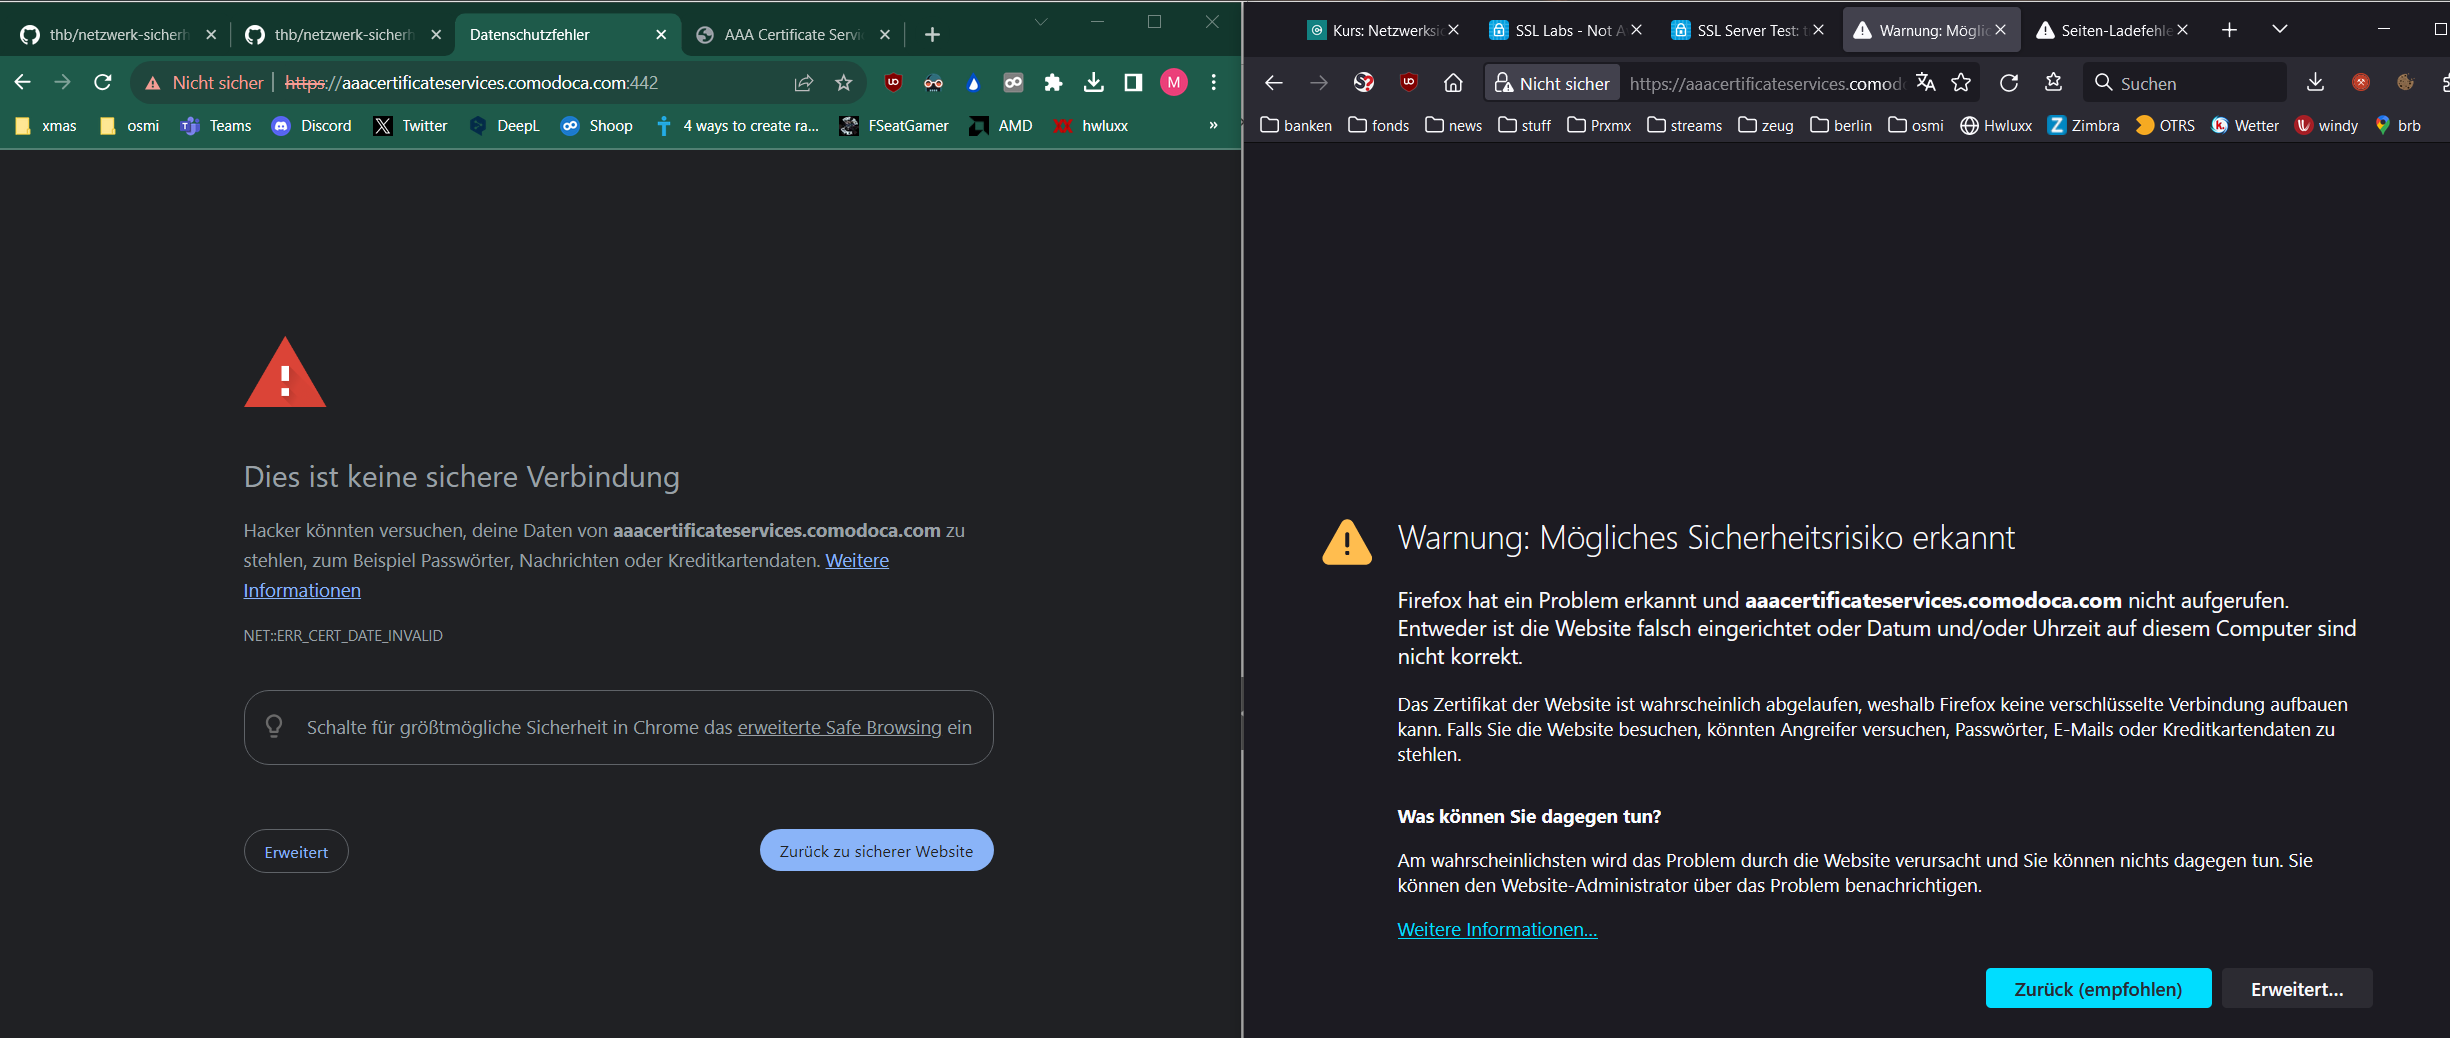
\includegraphics[width=0.75\textwidth]{images/05}
	\centering
	\caption{Google Chrome vs Firefox – 442 – Unsafe / Unsafe}
\end{figure}

Bei diesem Web-Server / Port erkennen beide Browser direkt ein abgelaufenes Zertifikat und warnen den
Nutzer davor, diese Webseite zu verwenden (da die Identität des Servers nicht sicher gestellt werden konnte).

\begin{figure}[H]
	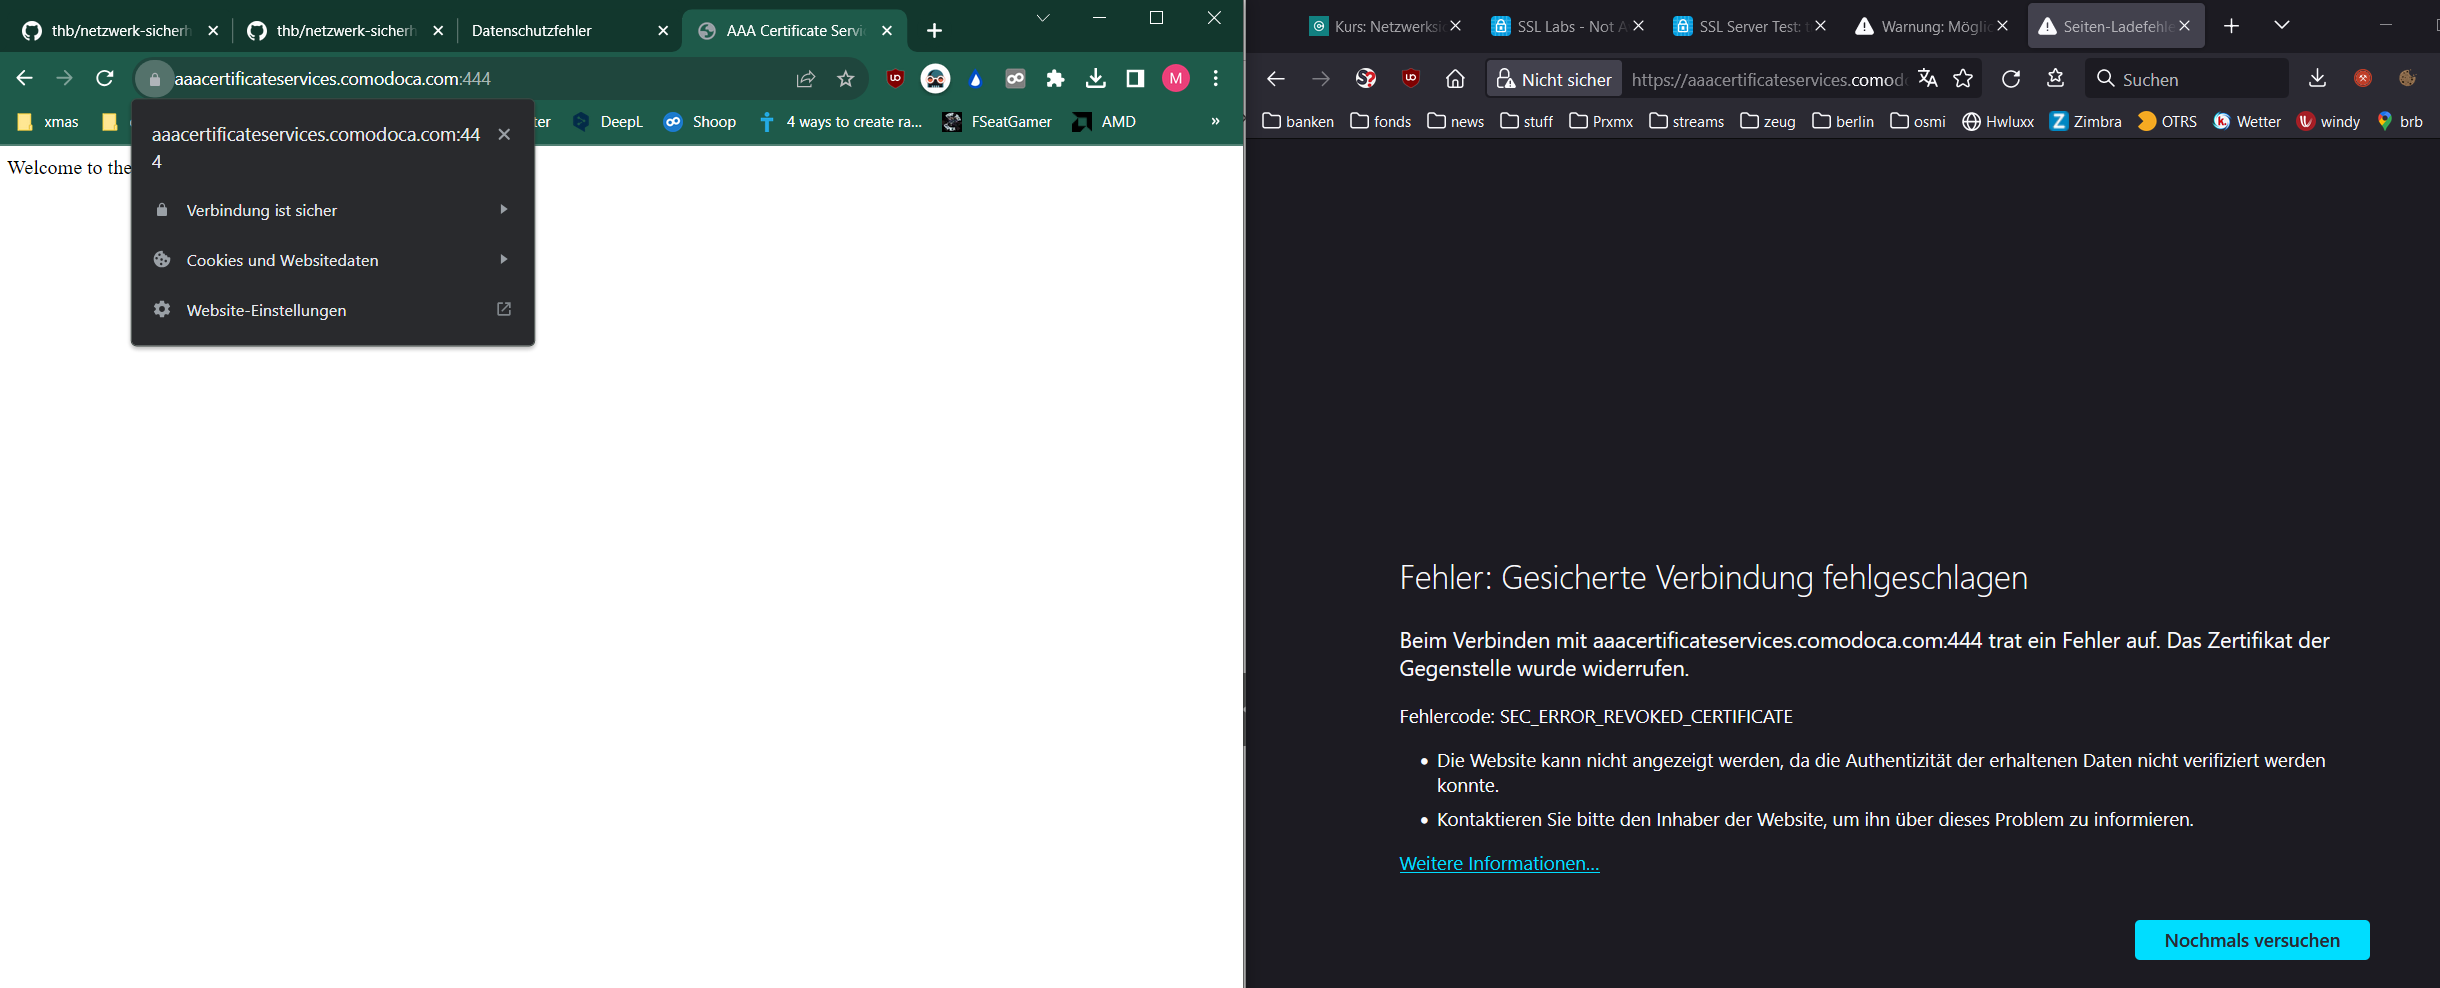
\includegraphics[width=0.75\textwidth]{images/06}
	\centering
	\caption{Google Chrome vs Firefox – 444 – Safe / Unsafe}
\end{figure}

Bei dem zweiten Test (also dem Server auf Port 444) verhalten sich die Browser interessanterweise unterschiedlich:
Chrome zeigt dies als sichere Verbindung an, obwohl Firefox warnt und angibt, dass das Zertifikat widerrufen worden sei.

\begin{figure}[H]
	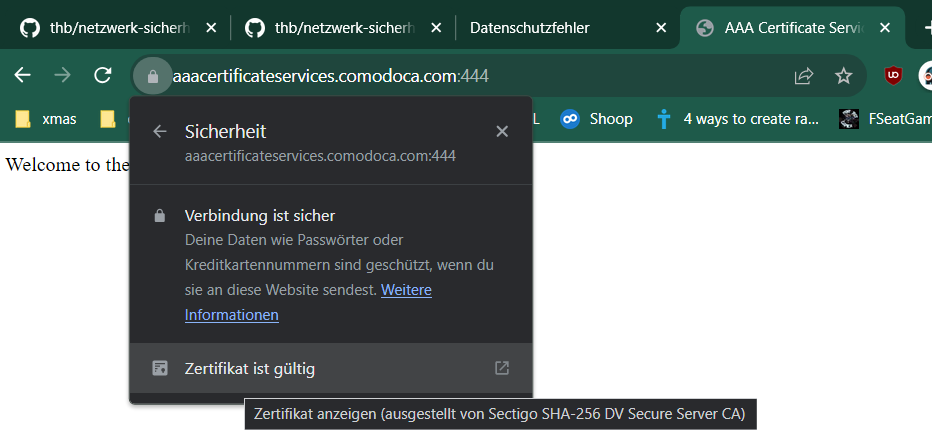
\includegraphics[width=0.75\textwidth]{images/07} 
	\centering
	\caption{Google Chrome vs Firefox – 444 – Details}
\end{figure}

\begin{figure}[H]
	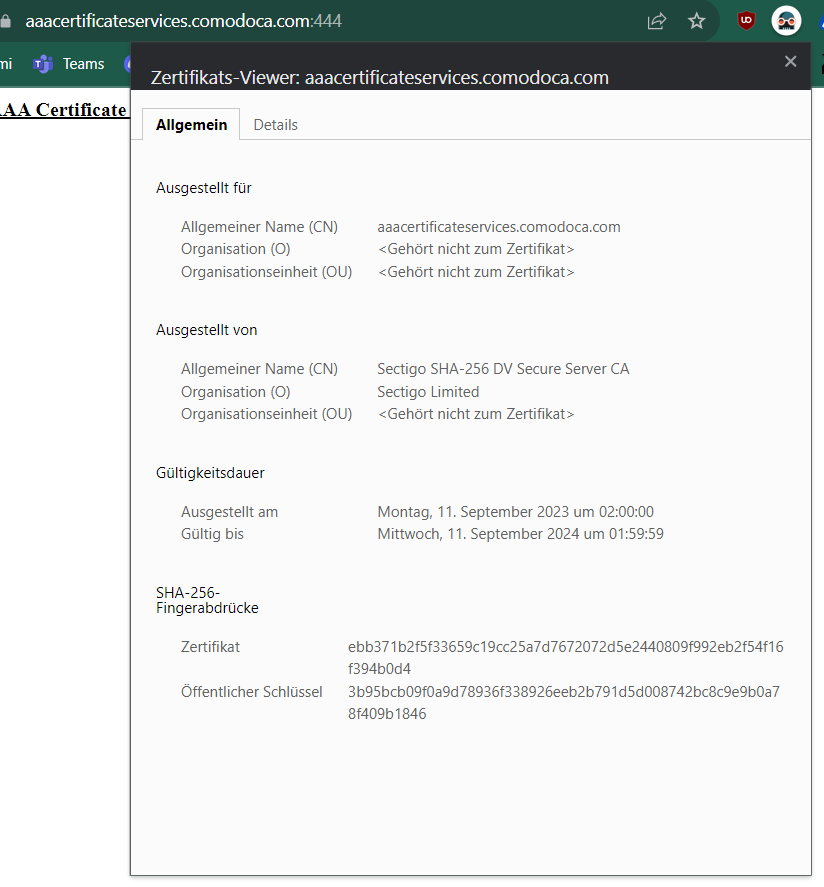
\includegraphics[width=0.75\textwidth]{images/08}
	\centering
	\caption{Google Chrome vs Firefox – 444 – Chrome Zertifikat}
\end{figure}

Auch bei näherer Betrachtung des Zertifikats im Chrome-Certificate-Viewer, lässt sich keine Spur von dem Widerruf finden.

Die unterschiedlichen Verhaltensweisen der Browser könnten mehrere Gründe haben:

\begin{enumerate}
  \item \textbf{CRL und OCSP}: Chrome und Firefox verwenden wahrscheinlich unterschiedliche Methoden zur Überprüfung des Widerrufsstatus eines Zertifikats. Chrome überprüft möglicherweise nicht den Widerrufsstatus oder konnte den Certificate Revocation List (CRL) oder Online Certificate Status Protocol (OCSP) Server nicht erreichen. Wenn der Server nicht erreichbar ist, kann Chrome die Verbindung unter bestimmten Bedingungen zulassen.
  \item \textbf{Caching}: Es könnte ein Caching-Problem vorliegen, bei dem Chrome das Zertifikat oder seinen Status zwischengespeichert hat und keinen Live-Check durchführt, um zu sehen, ob das Zertifikat widerrufen wurde.
  \item \textbf{Widerrufsinformationen}: Es ist auch möglich, dass Firefox aktualisierte Widerrufsinformationen hat, die Chrome nicht hat. Dies kann passieren, wenn die Widerrufsinformationen kürzlich aktualisiert wurden und Chrome das Update noch nicht erhalten hat.
  \item \textbf{Browser-Konfiguration}: Die Sicherheitseinstellungen des Browsers könnten unterschiedlich konfiguriert sein. Zum Beispiel könnte Chrome so eingerichtet sein, dass es mit bestimmten Arten von Zertifikatsfehlern fortfährt, die Firefox nicht zulässt, oder umgekehrt.
  \item \textbf{Certificate Pinning}: Chrome könnte das Zertifikat für diese Seite gepinnt haben, was die normale Überprüfung der Vertrauenskette umgehen würde, die sonst zu einer erkannten Widerrufsstatus führen könnte.
\end{enumerate}

Da wir allerdings beide Browser kontrollieren und beide Browser zum Zeitpunkt des Tests auf dem neusten Stand waren und wir den Web-Server vorher noch nie
verwendet haben, deutet dies auf eine Diskrepanz bei den CRL / OSCP Abfragen hin – wahrscheinlich, da unterschiedliche Informationen verwendet werden.

In einem solchen Fall, sollte immer dem Browser mit Sicherheitsbedenken vertraut werden.

\newpage

\subsection{Verschlüsselung}

\subsubsection*{Aufgabenstellung}

Installieren Sie VeraCrypt  auf Ihrem Rechner. Hierzu erhalten Sie zusätzlich eine 
VeraCrypt-Datei. In der Datei ist ein normaler und ein versteckter Container 
zu finden, die jeweils eine Datei enthalten. Das Passwort für den normalen 
Container ist der Exponent e des RSA-Schlüssels vom nwsmooc.mooin.org-Server. 
Dokumentieren Sie Ihre Vorgehensweise mit Screenshots und geben Sie 
anschließend das im versteckten Container gefundene Kennwort an.

Hinweis: Zur Bedienung von VeraCrypt können Sie sich beispielsweise hier ein Video 
ansehen: https://youtu.be/atb2pdxd394.

\subsubsection*{Antwort}

Um das zur Verfügung gestellte VeraCrypt File öffnen zu können, soll der Exponent 
$e$ des RSA-Schlüssels der Webseite \texttt{nwsmooc.mooin.org} verwendet werden. 
Diesen Exponenten kann man sich ganz einfach ausgeben lassen, in dem man sich im 
Mozilla Firefox Browser jene Webseite öffnet und auf das Schlosssymbol drückt, um 
sich das Zertifikat anzusehen.

\begin{figure}[H]
	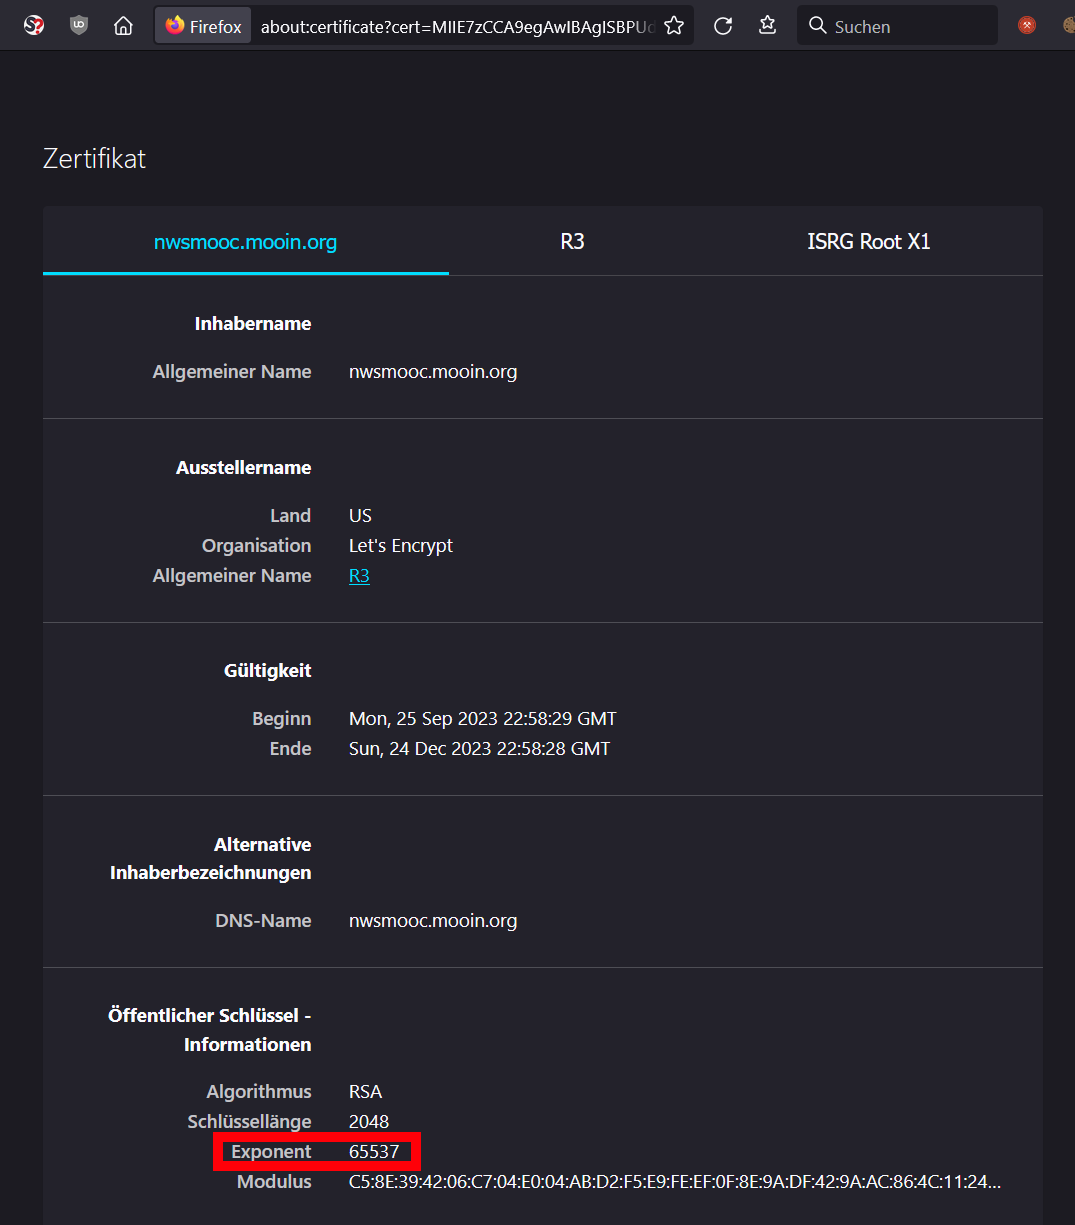
\includegraphics[width=0.675\textwidth]{images/09}
	\centering
	\caption{Vercrypt – Exponent}
\end{figure}

Im Abschnitt ``Öffentlicher Schlüssel – Informationen'' bekommt man den Exponenten 
des öffentlichen Schlüssels ausgegeben (siehe Abb. 9). Allerdings gelang uns der 
Zugriff auf den Container auch vor der Analyse des Zertifikats, da $e = 65537_{10}$ 
in der Praxis üblich ist.

Für das RSA Verfahren werden große Primzahlen bevorzugt verwendet und der 
Algorithmus muss dabei unterschiedliche Operationen bei der Bearbeitung basierend 
auf dem Binärcode tätigen. Da $65537_{10} = 10000000000000001_2$ führt 
dies zu einer effizienten Arbeitsweise des Algorithmus – Einsen werden 
multipliziert, Nullen potenziert.

\begin{figure}[H]
	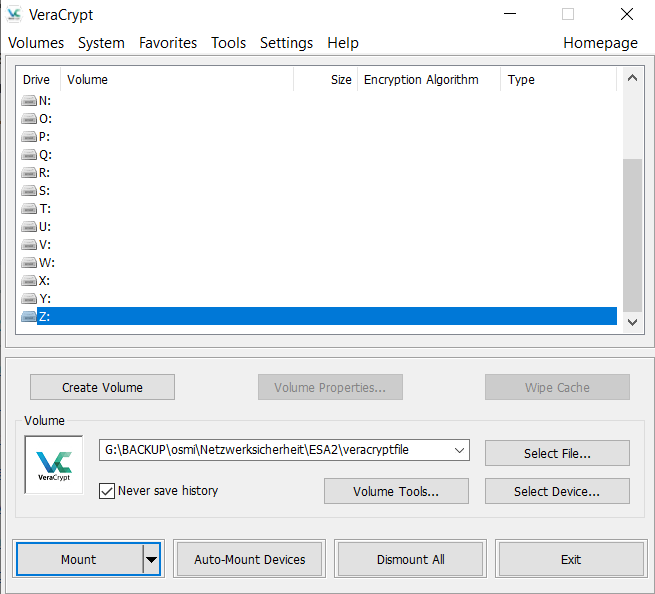
\includegraphics[width=0.75\textwidth]{images/10}
	\centering
	\caption{Vercrypt – Einbinden Container}
\end{figure}

\begin{figure}[H]
	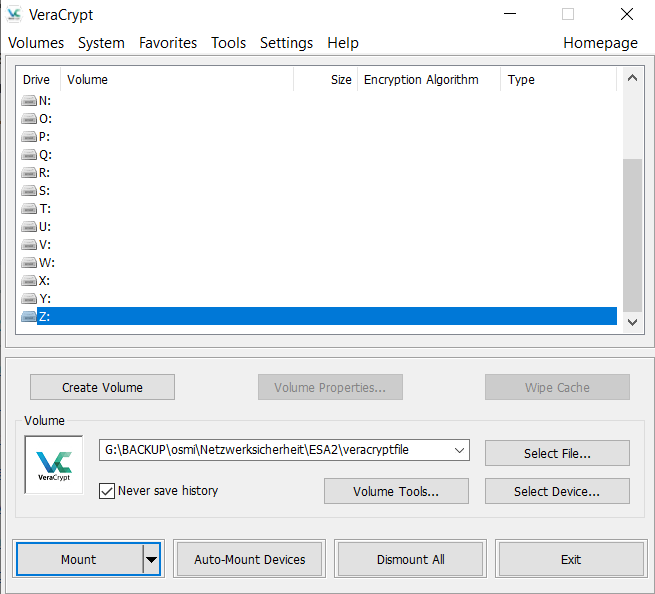
\includegraphics[width=0.75\textwidth]{images/11}
	\centering
	\caption{Vercrypt – Passworteingabe}
\end{figure}

Nun können wir mit VeraCrypt (unter Angabe des Passworts 65537) die im Kurs 
bereitgestellte Datei als Laufwerk einbinden und somit Zugriff auf den Inhalt 
erhalten.

\begin{figure}[H]
	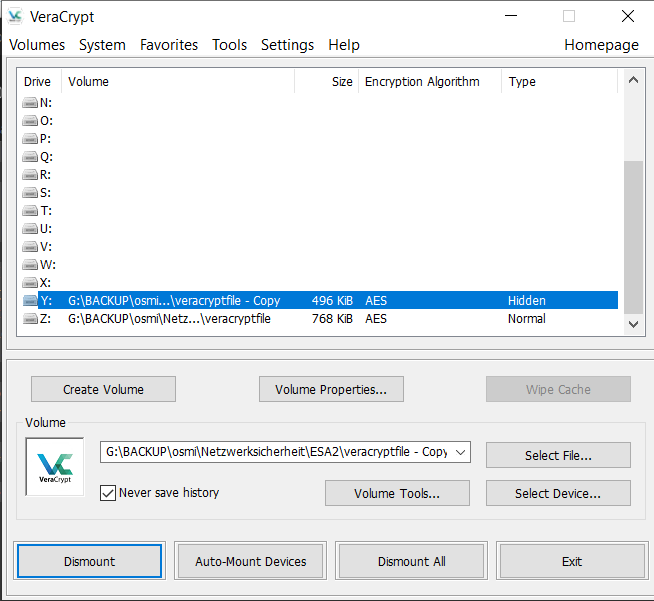
\includegraphics[width=0.75\textwidth]{images/12}
	\centering
	\caption{Vercrypt – Einbinden Versteckter Container}
\end{figure}

Die enthaltene Textdatei ``Datei-angezeigter-Container.txt'' lautet: ``Das 
Zugangskennwort für den versteckten Container lautet: 	VerSteCon0815''

\begin{figure}[H]
	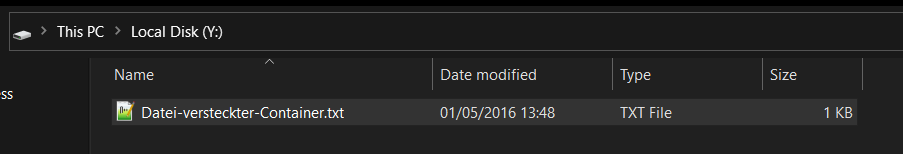
\includegraphics[width=0.75\textwidth]{images/13}
	\centering
	\caption{Vercrypt – Versteckter Container}
\end{figure}

Wir konnten uns an das Modul Digitaler Selbstschutz erinnern, in dessen Report-
Inhalt VeraCrypt bereits vorkam, und haben den Container kopiert und ein 2. Mal 
eingebunden, wobei dieses Mal das Passwort ``VerSteCon0815'' eingegeben werden muss 
um Zugriff auf den versteckten Container zu erhalten.

Somit konnten wir Zugriff auf den versteckten Container und seinem Inhalt ``Datei-
versteckter-Container.txt'' erlangen und den Inhalt auslesen: 
``HiddenVolumeVeraCrypt''.

\newpage

\subsection{Steganographie}

\subsubsection*{Aufgabenstellung}

Installieren Sie SilentEye  auf Ihrem Rechner und untersuchen Sie die 
bereitgestellten Beispieldateien. mooin.jpg enthält ein verstecktes Kennwort, 
mooin.bmp eine Datei. Die notwendigen Einstellungen können Sie der Aufgabe mit 
VeraCrypt entnehmen. Dokumentieren Sie Ihre Vorgehensweise mit Screenshots und 
geben Sie das gefundene Kennwort an.

Hinweis: Sollte es Schwierigkeiten geben, wenn Sie beide Dateien nacheinander 
untersuchen, dann schließen Sie SilentEye zwischendurch.

\subsubsection*{Antwort}

\begin{figure}[H]
	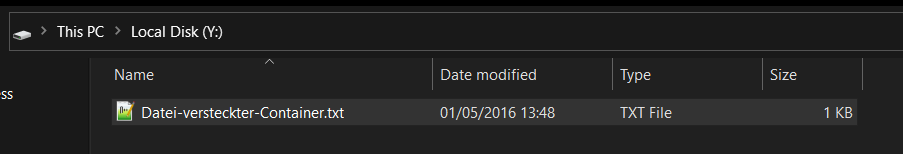
\includegraphics[width=0.75\textwidth]{images/14}
	\centering
	\caption{Vercrypt – Hidden Container}
\end{figure}

% Die Einstellungen von SilentEye, die Sie für die Fortgeschrittenenaufgabe brauchen, 
% sind:

% Key (für beide Dateien): NWSMOOC_Test
% Passphrase (nur für jpg-Datei): SilentEye_Test

Die anderen Einstellungen entsprechen den Default-Einstellungen

Für mooin.jpg: 
Luminance Interval = 5 
Header Position = bottom
CharSet = UTF8

Für mooin.bmp (Oben beim "Media's encoding format" auf "BMP" wechseln):
Image quality: 96,975% (normal); keine Veränderungen bei "Advanced"
Aktivieren Sie zusätzlich zu "Compressed Data" jeweils auch "Encrypted Data" mit AES256. Dort muss der Key in beide Kästchen eingetragen werden.
Über die SilentEye-Aufgabe erhalten Sie über mooin.bmp übrigens schon vorab eine Aufgabensammlung zur Klausurvorbereitung.

---

ÜBERARBEITEN

SilentEye ist eine Open-Source-Software, die zur Steganographie verwendet wird, um 
zusätzliche Informationen in Bildern und Audiodateien zu verstecken oder auszulesen. 

Um mooin.jpg zu untersuchen, öffnen wir die Datei mit dem Programm Silenteye und 
verwenden die Einstellungen aus der Lösung der Aufgabe 1.4.

Dadurch kann der verborgene Bereich des Bildes erfolgreich entschlüsselt werden und 
gibt als dekodierte Message den Text ``Kennwort: SteganographieInNWSMOOC'' frei.

Mit diesem Kennwort und den bereitgestellten Einstellungen für das zweite Bild, lässt 
sich auch dessen versteckter Inhalt sichtbar machen und entschlüsseln. Wir können an 
dieser Stelle die Datei AufgabensammlungSS16.pdf extrahieren und abspeichern.

\end{document}
